\appendix
\section*{Appendix A: Repository and previous-work context}
\phantomsection
\label{sec:appendix_repository_previous_work}
\addcontentsline{toc}{section}{Appendix A: Repository and previous-work context}

The active implementation used in this report is the COMSOL source-case pipeline developed during this project. The public project repository stores the reproducible parts of the work, including the source code, active TOML case definitions, report notes, plotting scripts, compact post-processing tables, and selected report figures \cite{KuijpersEWSComsolGitHub}. Large COMSOL build and solve artefacts are not part of the intended repository content because individual MPH files and recovery folders can become several gigabytes per case.

This work was developed in the context of previous EWS finite element modelling work. Ryan Engels' earlier FEBio-based model provided a useful reference for the older soft-tissue modelling route and displacement-based evaluation \cite{EngelsEWSReport}. Femke Storm's Sioux/EWS work provided additional context for soft material settings, skin representation, and an HGO-like adipose reinforcement concept for Cooper-like support \cite{StormEWSReport}. These documents were used as internal project context and engineering comparison material. They are therefore cited separately from peer-reviewed literature and should not be interpreted as independent validation sources.

The main difference between the current repository and the earlier FEBio-oriented work is the implementation strategy. The current route emphasizes COMSOL geometry generation, boolean region construction, automatic selections, build-only checks, and structured case management through TOML files. The older FEBio route remains useful for comparison, especially for material choices and expected dynamic response ranges, but the active model development and report figures are based on the COMSOL pipeline.

\section*{Appendix B: Figure and metric sources}
\phantomsection
\label{sec:appendix_figures}
\addcontentsline{toc}{section}{Appendix B: Figure and metric sources}

This appendix records the generated contact-sheet figures used in the report. The complete source index is stored in \texttt{docs/report\_notes/comsol\_pipeline/report\_figures\_metrics\_index.md}; it lists the exact COMSOL output folders, metric JSON files, and source PNG panels used for each contact sheet.

\begin{figure}[H]
\centering
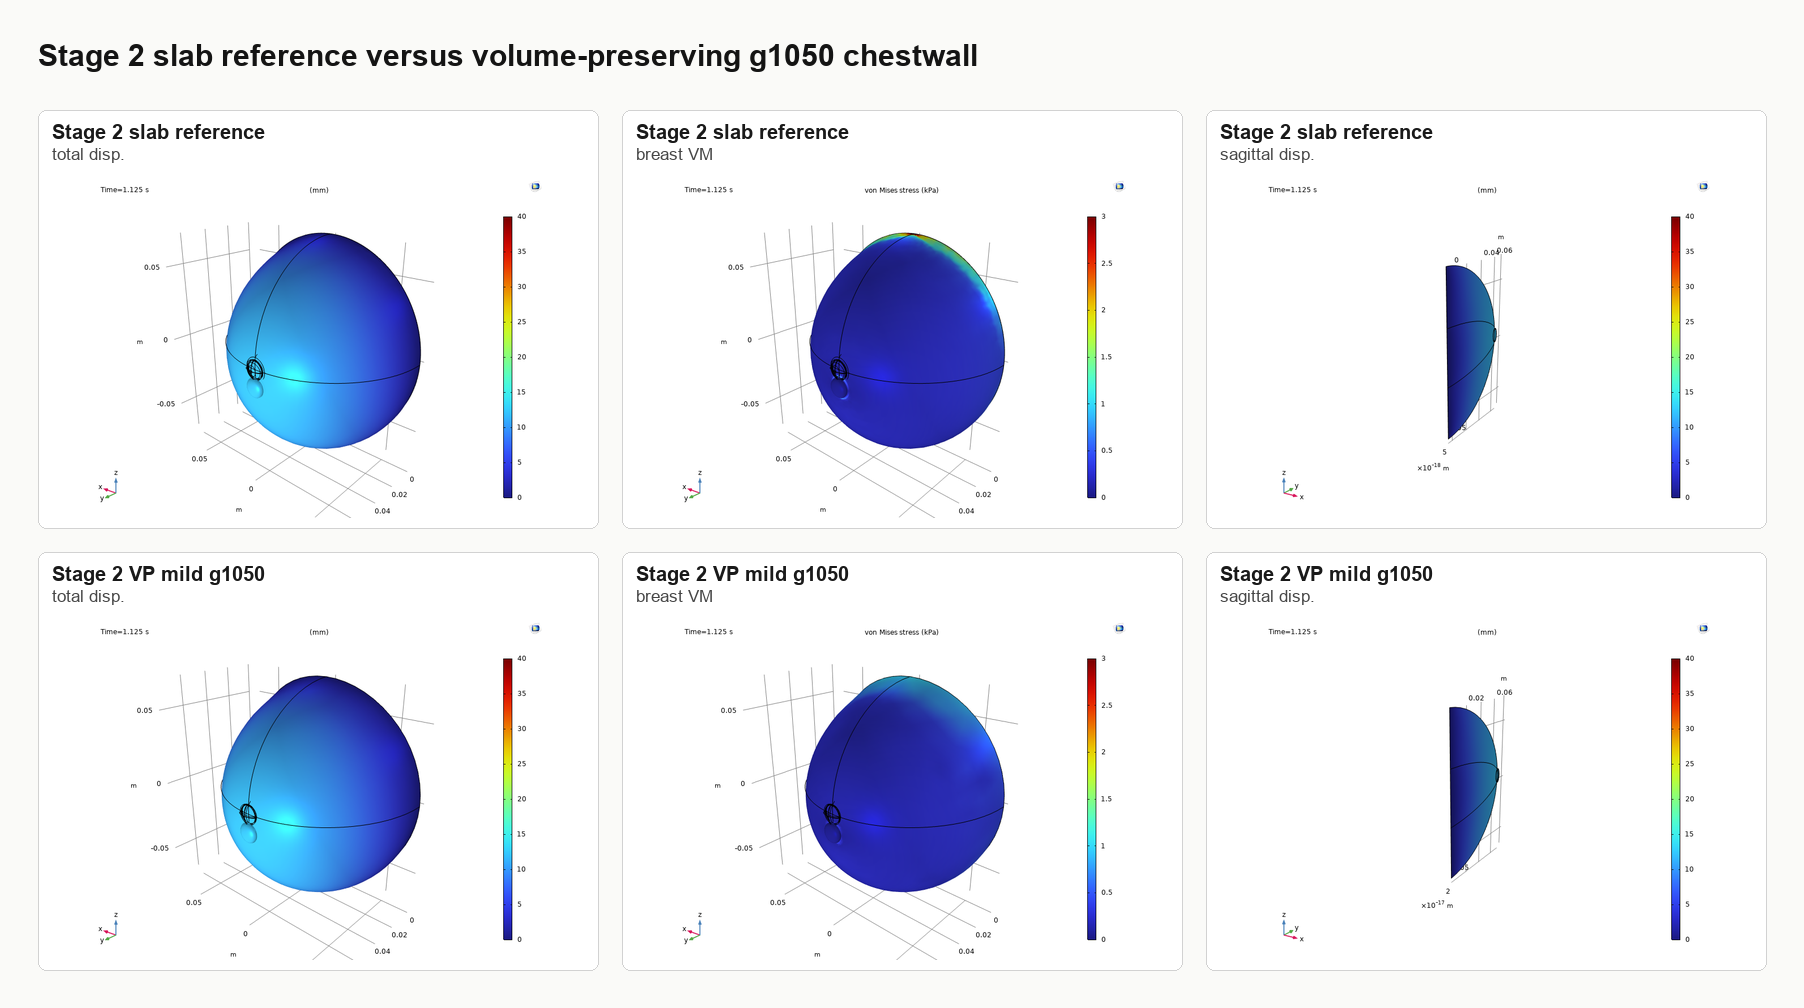
\includegraphics[width=0.95\linewidth,height=0.78\textheight,keepaspectratio]{Figures/comsol_contact_sheets/stage2_chestwall_contact_sheet.png}
\caption{Stage 2 support-geometry source figure using displacement and von Mises stress panels.}
\label{fig:appendix_stage2_figures}
\end{figure}

\begin{figure}[H]
\centering
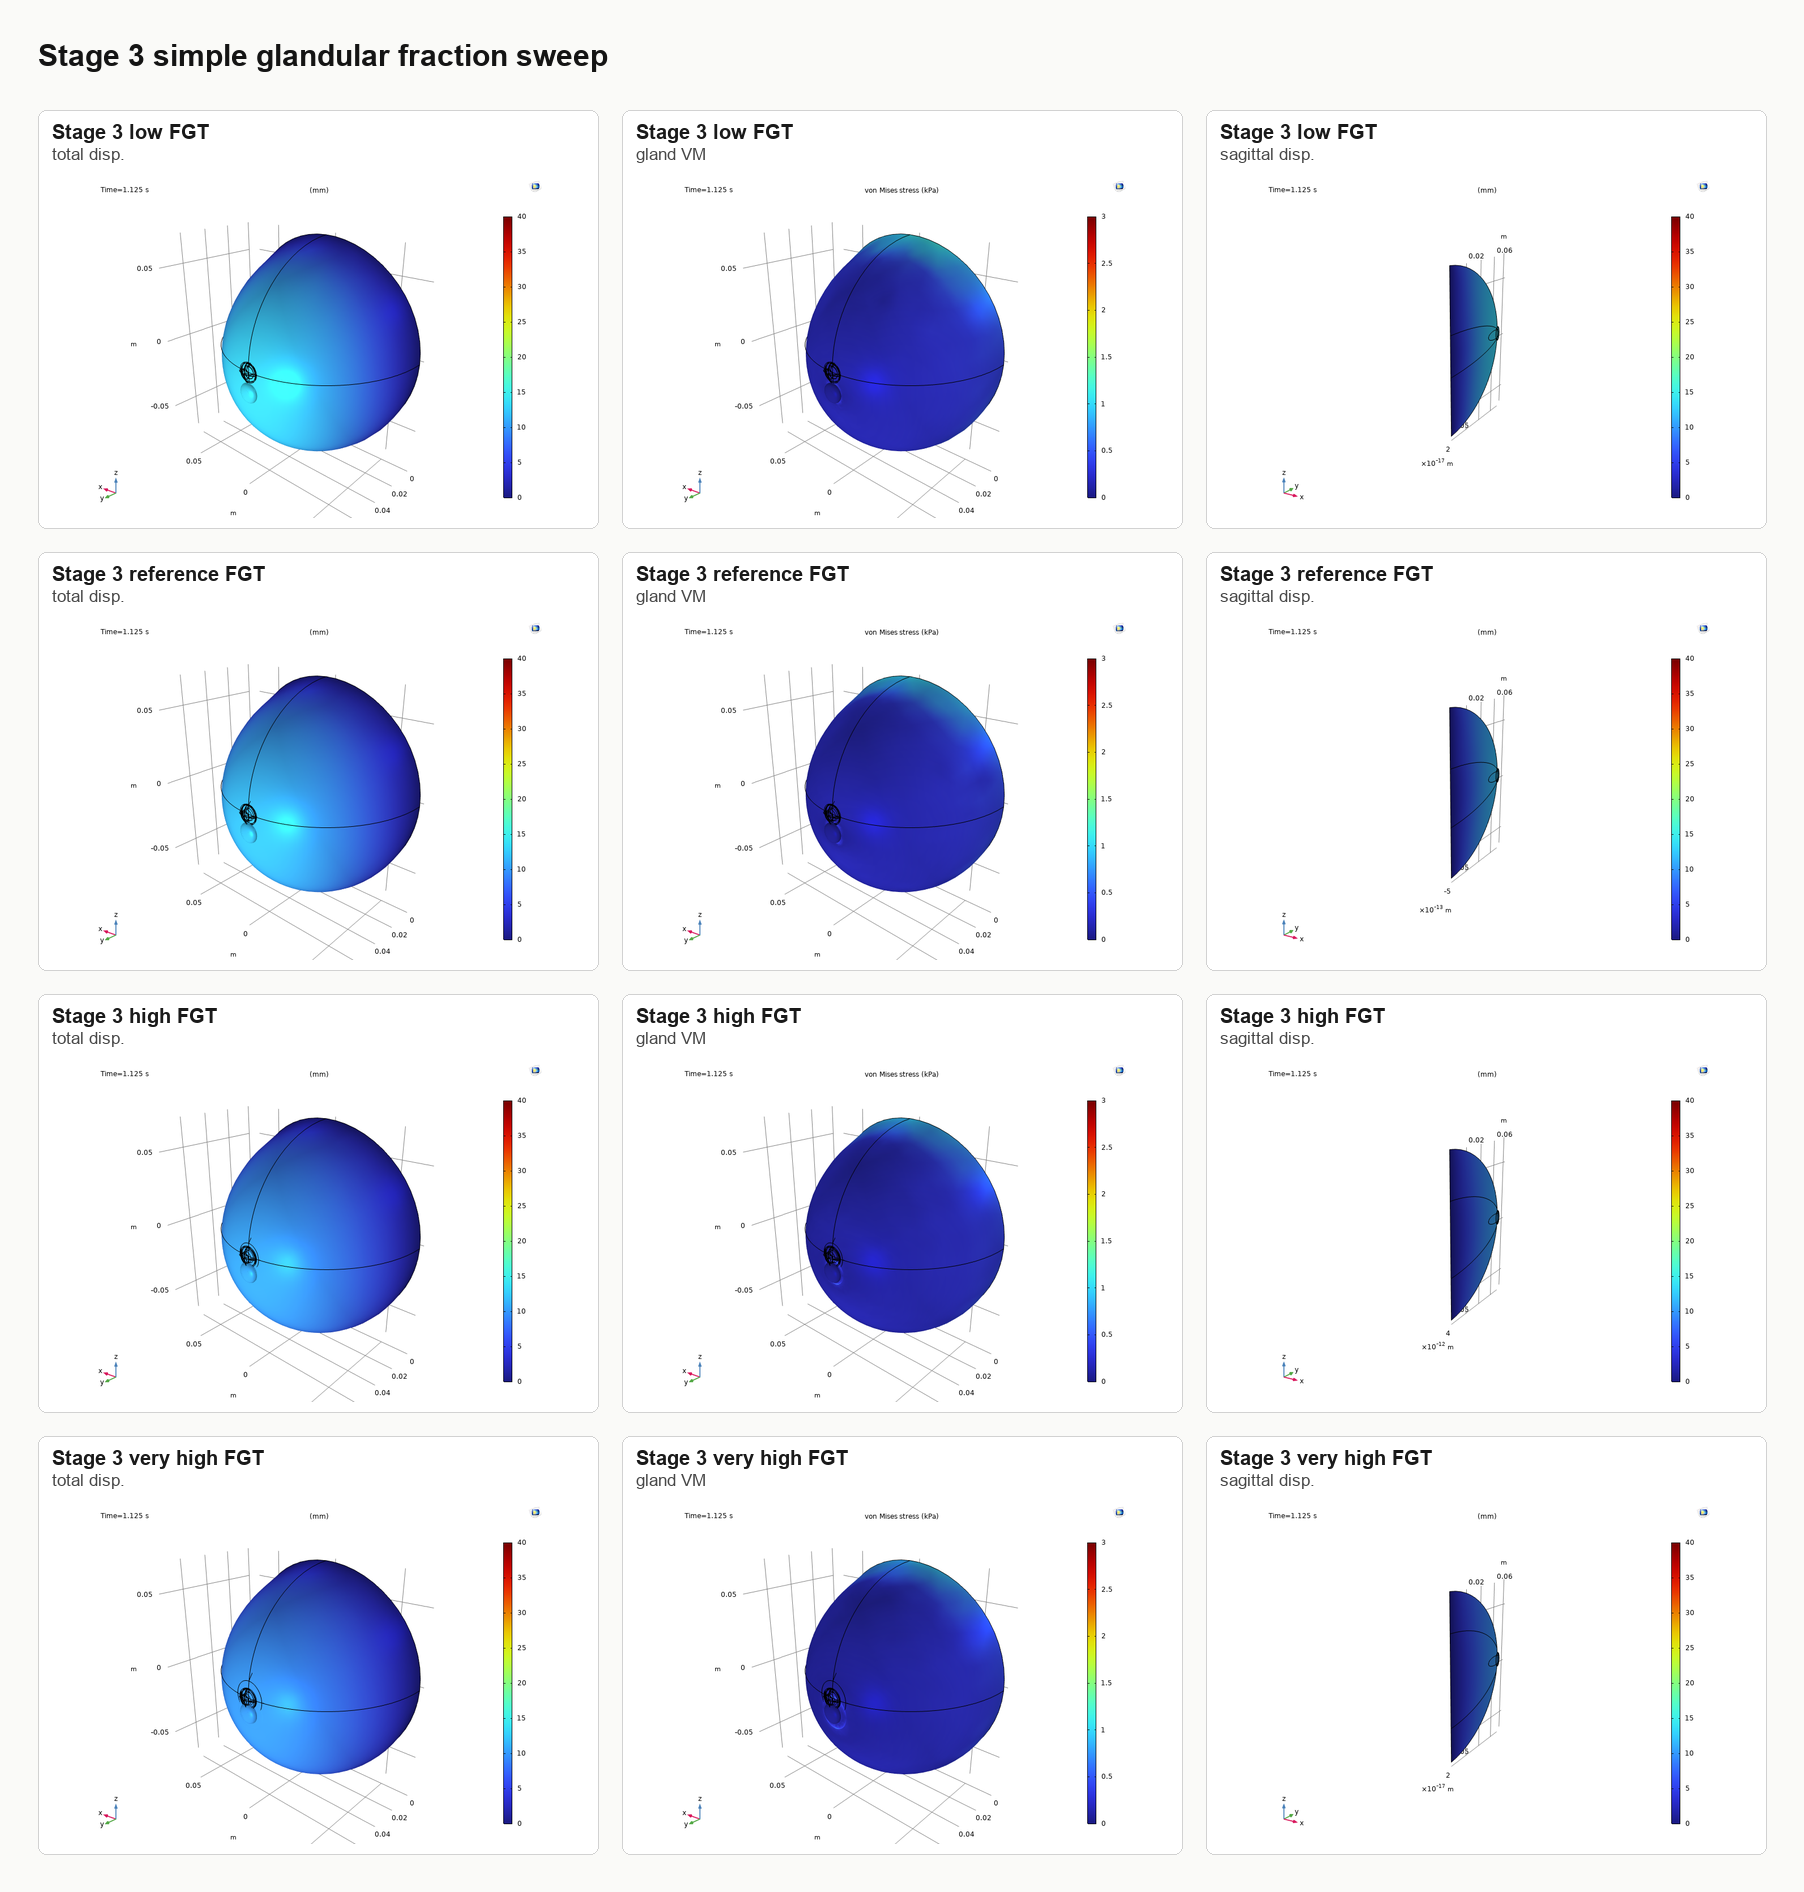
\includegraphics[width=0.95\linewidth,height=0.78\textheight,keepaspectratio]{Figures/comsol_contact_sheets/stage3_glandular_fraction_contact_sheet.png}
\caption{Stage 3 source figure comparing the solved simple glandular fraction sensitivity.}
\label{fig:appendix_stage3_fraction_figures}
\end{figure}

\begin{figure}[H]
\centering
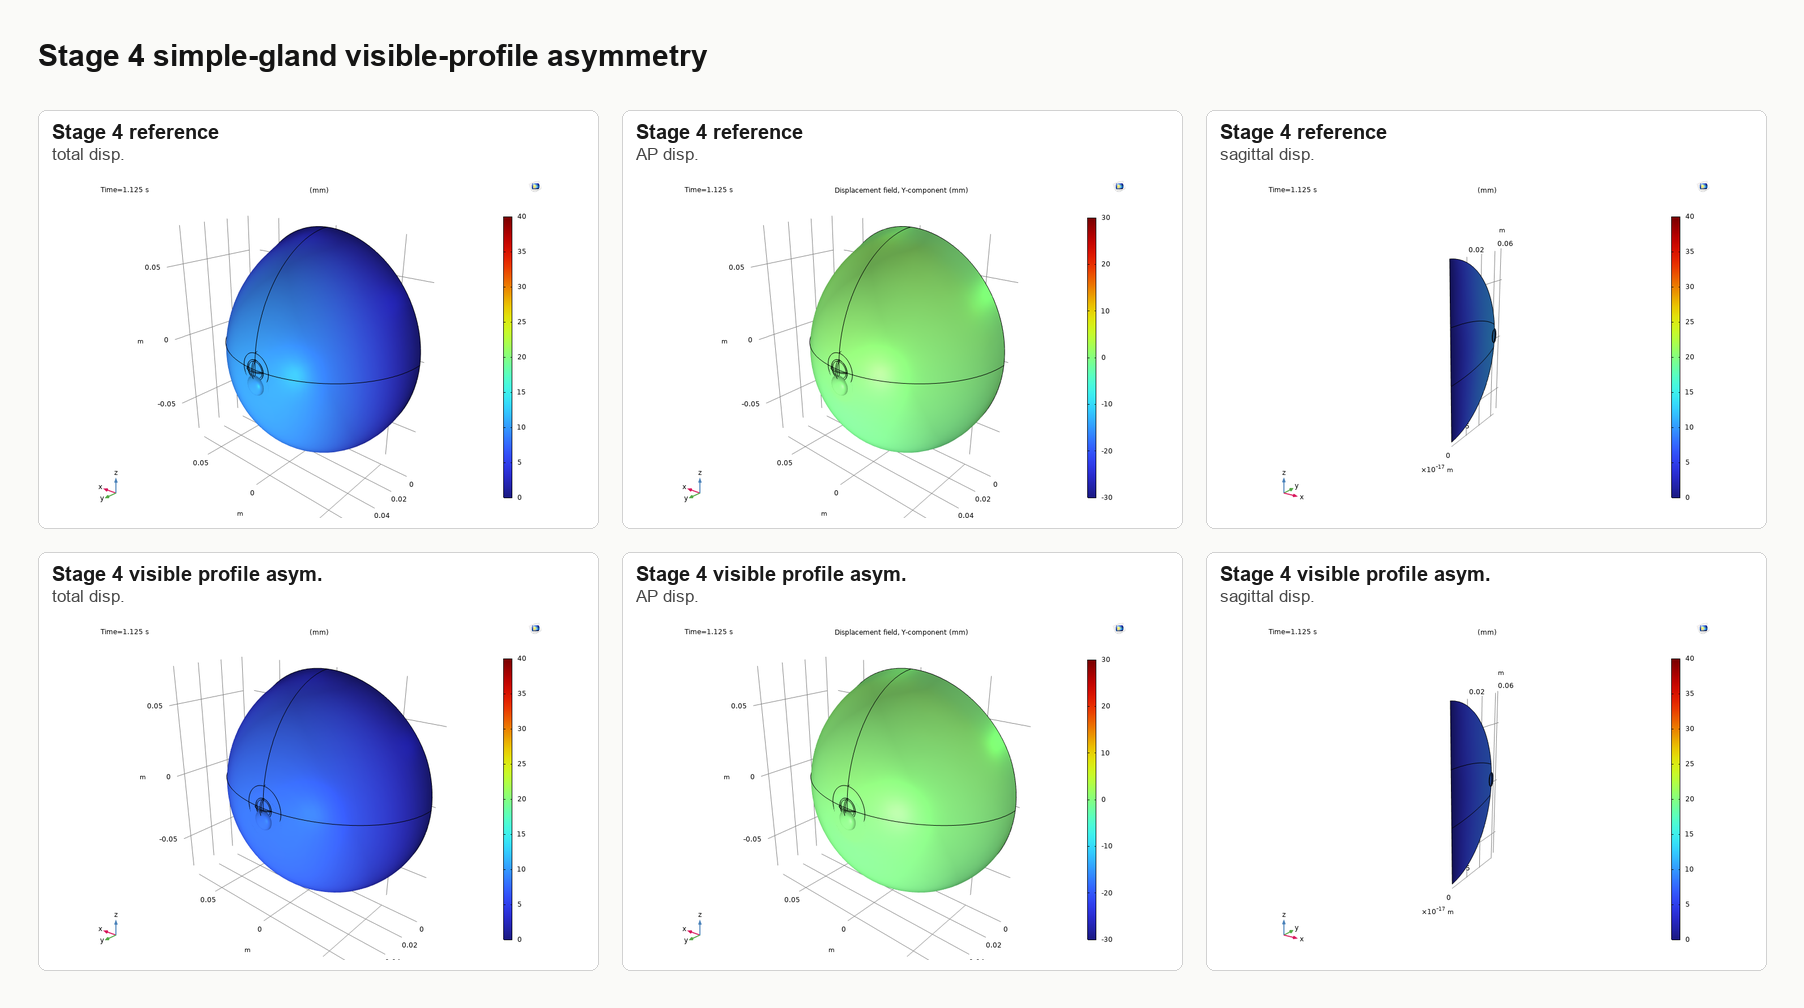
\includegraphics[width=0.95\linewidth,height=0.78\textheight,keepaspectratio]{Figures/comsol_contact_sheets/stage4_asymmetry_contact_sheet.png}
\caption{Stage 4 source figure comparing the simple-gland reference and the clean visible-profile asymmetry case.}
\label{fig:appendix_stage4_figures}
\end{figure}

\begin{figure}[H]
\centering
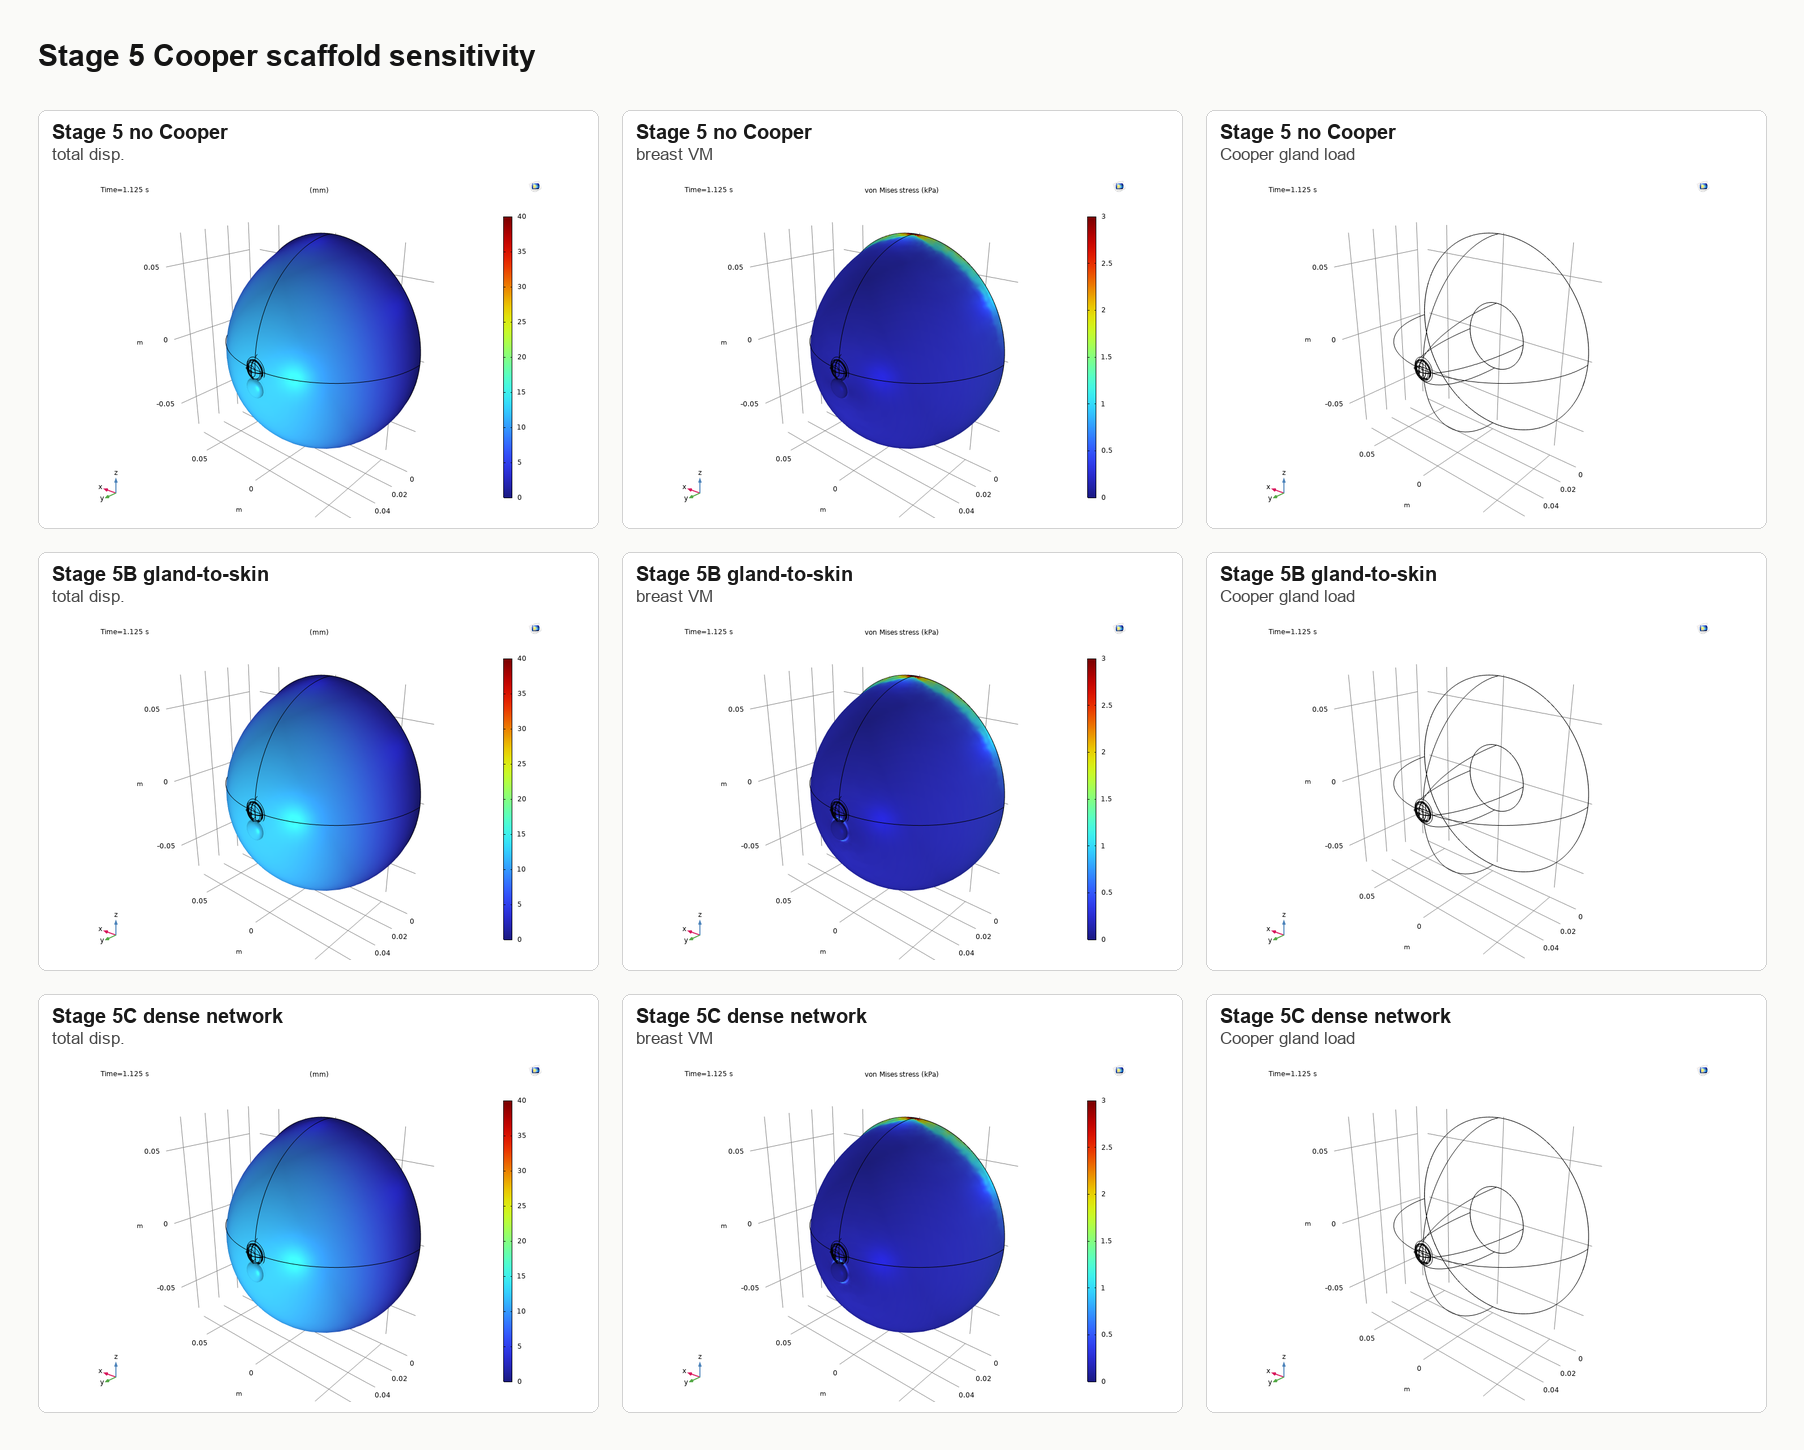
\includegraphics[width=0.95\linewidth,height=0.78\textheight,keepaspectratio]{Figures/comsol_contact_sheets/stage5_cooper_contact_sheet.png}
\caption{Stage 5 source figure for the Cooper-support development branch. The current robust Tier 1 interpretation uses the no-Cooper control; Cooper-support effects require a stable solved variant before being treated as report-ready.}
\label{fig:appendix_stage5_figures}
\end{figure}

\section*{Appendix C: Run-status notes}
\phantomsection
\label{sec:appendix_status}
\addcontentsline{toc}{section}{Appendix C: Run-status notes}

The current report distinguishes between solved report-ready cases, control cases, and exploratory cases. Stage 1 is a motion sanity baseline rather than the final anatomical reference. Stage 2 is the first fair anatomical baseline. Stage 3 is the current realistic glandular reference, while Stage 4 and Stage 5 are currently interpreted as no-asymmetry and no-Cooper controls in the Tier 1 comparison. Stage 6 tumor cases should only be used quantitatively after complete tumor-mask metrics are available. The older Stage 4 additive lateral/fullness ellipsoid cases should not be used as report evidence because the helper ellipsoids were included as separate volumes in the final breast union.

\section*{Appendix D: Breast-volume dataset summary}
\phantomsection
\label{sec:appendix_volume_summary}
\addcontentsline{toc}{section}{Appendix D: Breast-volume dataset summary}

The table below summarizes the 100-sample breast-volume dataset used to benchmark the COMSOL model volume range. The contours were drawn approximately 5 mm inside the outer breast boundary and in a lying/supine-like position, so these values should be interpreted as conservative internal-envelope volumes rather than full external breast volumes. The detailed literature comparison is stored in \texttt{docs/report\_notes/comsol\_pipeline/model\_justification/breast\_volume\_literature\_context\_2026-05-26.md}.

\begin{table}[H]
\centering
\caption{Summary statistics of the 100-sample breast-volume dataset.}
\label{tab:appendix_breast_volume_dataset}
\begin{tabular}{lr}
\hline
Statistic & Volume (ml) \\
\hline
Number of samples & 100 \\
Minimum & 105.68 \\
10th percentile & 363.86 \\
25th percentile (Q1) & 519.65 \\
Median & 691.15 \\
Mean & 728.32 \\
75th percentile (Q3) & 928.70 \\
90th percentile & 1135.46 \\
Maximum & 1777.28 \\
Standard deviation & 327.39 \\
IQR & 409.05 \\
\hline
\end{tabular}
\end{table}

\section*{Appendix E: Stage 6 tumor candidate definitions}
\phantomsection
\label{sec:appendix_stage6_tumor_candidates}
\addcontentsline{toc}{section}{Appendix E: Stage 6 tumor candidate definitions}

The table below records the current Stage 6 tumor-screening candidates. Positions are COMSOL model coordinates in metres. These cases use the analytic spherical \texttt{tumor\_mask}; they should therefore be interpreted as internal material-overlay sensitivity cases rather than separate segmented tumor geometries.

\begin{table}[H]
\centering
\small
\caption{Current Stage 6 tumor candidate definitions for build-screening and fast dynamic evaluation.}
\label{tab:appendix_stage6_tumor_candidates}
\begin{tabular}{p{0.28\linewidth} p{0.15\linewidth} p{0.22\linewidth} p{0.25\linewidth}}
\toprule
Candidate & Diameter & Position $(x,y,z)$ & Purpose \\
\midrule
No-tumor control & -- & -- & Matched Stage 6 reference without lesion overlay. \\
Small central & 6 mm & central reference & First local stiffness probe. \\
Medium central & 12 mm & central reference & Size sensitivity with moderate lesion. \\
Large central & 20 mm & central reference & Upper T1-size diagnostic sensitivity; use cautiously. \\
Small upper-outer & 6 mm & upper-outer reference & Most common-quadrant location probe. \\
Small subareolar & 6 mm & anterior/subareolar & Nipple/landmark sensitivity probe. \\
Small posterior & 6 mm & chestwall-proximal & Deep lesion detectability probe. \\
Small upper-outer surface-proximal & 6 mm & (0.025, 0.060, 0.018) & Inner-surface proximity probe. \\
Small upper-outer superior & 6 mm & (0.025, 0.050, 0.040) & Superior upper-outer placement probe. \\
Medium upper-outer surface-proximal & 12 mm & (0.025, 0.056, 0.018) & Size and surface-proximity sensitivity. \\
Medium upper-outer superior & 12 mm & (0.025, 0.046, 0.040) & Size and superior-location sensitivity. \\
Mild/stiff tumor variants & case-specific & usually central or upper-outer & Material stiffness sensitivity. \\
\bottomrule
\end{tabular}
\end{table}

The most report-useful first dynamic comparison is not the full list above, but a compact subset: no-tumor control, small central, small upper-outer, small subareolar, small posterior, and one surface-proximal upper-outer candidate. Medium and large cases are most useful after the small cases show stable tumor-mask volume and measurable local metrics.

\section*{Appendix F: Model-geometry screenshots}
\phantomsection
\label{sec:appendix_model_geometry_screens}
\addcontentsline{toc}{section}{Appendix F: Model-geometry screenshots}

This appendix is reserved for the manually captured COMSOL geometry screenshots. These images document what changed between model stages and are separate from the automated displacement and stress contact sheets. The files are expected under \texttt{Figures/model\_pictures/} in the final report folder.

\begin{figure}[H]
\centering
\begin{subfigure}{0.48\linewidth}
\centering
\IfFileExists{Figures/model_pictures/stage2_chestwall/stage2_chestwall_superior_transversal_offset055.png}{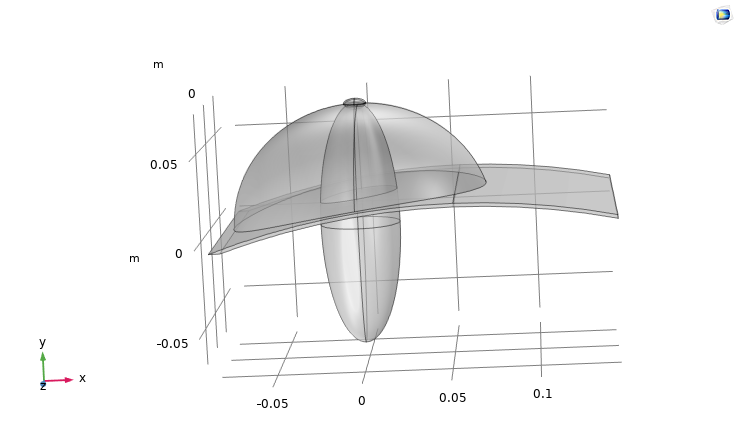
\includegraphics[width=\linewidth]{Figures/model_pictures/stage2_chestwall/stage2_chestwall_superior_transversal_offset055.png}}{\fbox{\parbox[c][0.24\textheight][c]{0.9\linewidth}{\centering Placeholder: Stage 2 superior transverse chestwall view}}}
\caption{Superior view}
\end{subfigure}
\hfill
\begin{subfigure}{0.48\linewidth}
\centering
\IfFileExists{Figures/model_pictures/stage2_chestwall/stage2_chestwall_leftlateral_offset055.png}{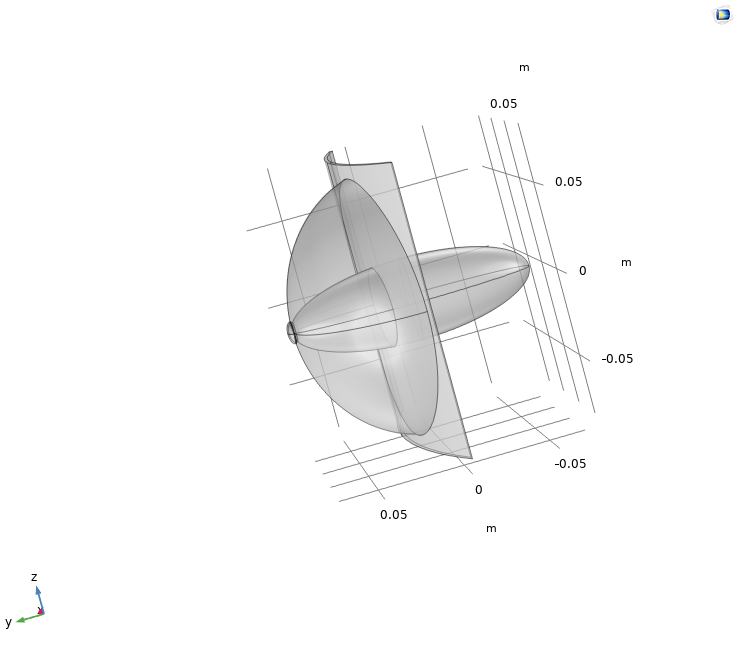
\includegraphics[width=\linewidth]{Figures/model_pictures/stage2_chestwall/stage2_chestwall_leftlateral_offset055.png}}{\fbox{\parbox[c][0.24\textheight][c]{0.9\linewidth}{\centering Placeholder: Stage 2 lateral chestwall view}}}
\caption{Lateral view}
\end{subfigure}
\caption{Stage 2 selected xoffset055 chestwall geometry. This figure is intended to show the posterior support curvature used as the first fair anatomical baseline.}
\label{fig:appendix_stage2_geometry_screens}
\end{figure}

\begin{figure}[H]
\centering
\begin{subfigure}{0.32\linewidth}
\centering
\IfFileExists{Figures/model_pictures/stage3_glandular/stage3_glandular_compact_anterior_offset055.png}{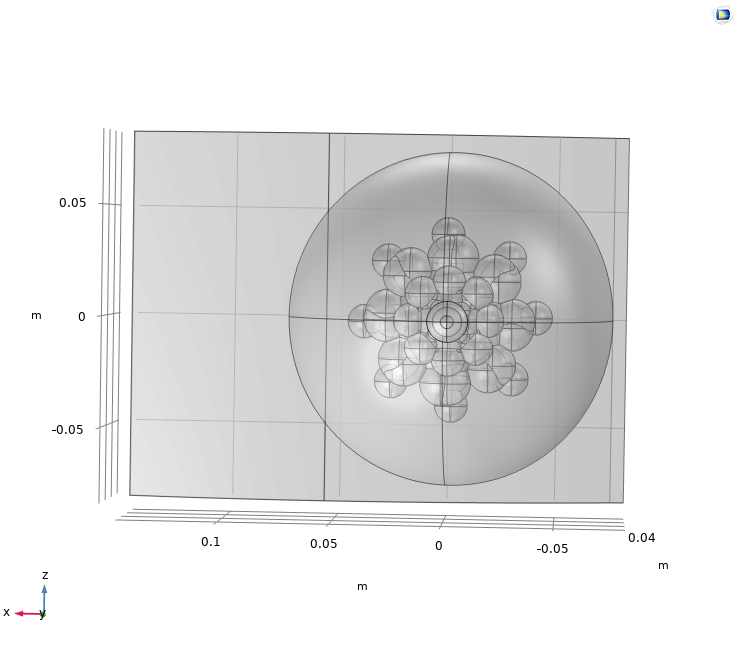
\includegraphics[width=\linewidth]{Figures/model_pictures/stage3_glandular/stage3_glandular_compact_anterior_offset055.png}}{\fbox{\parbox[c][0.2\textheight][c]{0.9\linewidth}{\centering Placeholder: compact glandular spread}}}
\caption{Compact}
\end{subfigure}
\hfill
\begin{subfigure}{0.32\linewidth}
\centering
\IfFileExists{Figures/model_pictures/stage3_glandular/stage3_glandular_ref_anterior_offset055.png}{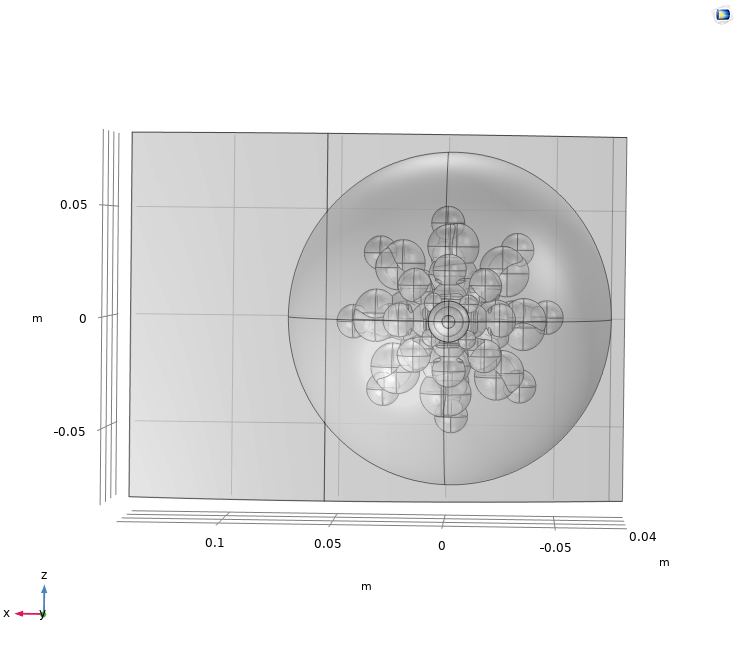
\includegraphics[width=\linewidth]{Figures/model_pictures/stage3_glandular/stage3_glandular_ref_anterior_offset055.png}}{\fbox{\parbox[c][0.2\textheight][c]{0.9\linewidth}{\centering Placeholder: reference glandular spread}}}
\caption{Reference}
\end{subfigure}
\hfill
\begin{subfigure}{0.32\linewidth}
\centering
\IfFileExists{Figures/model_pictures/stage3_glandular/stage3_glandular_wide_anterior_offset055.png}{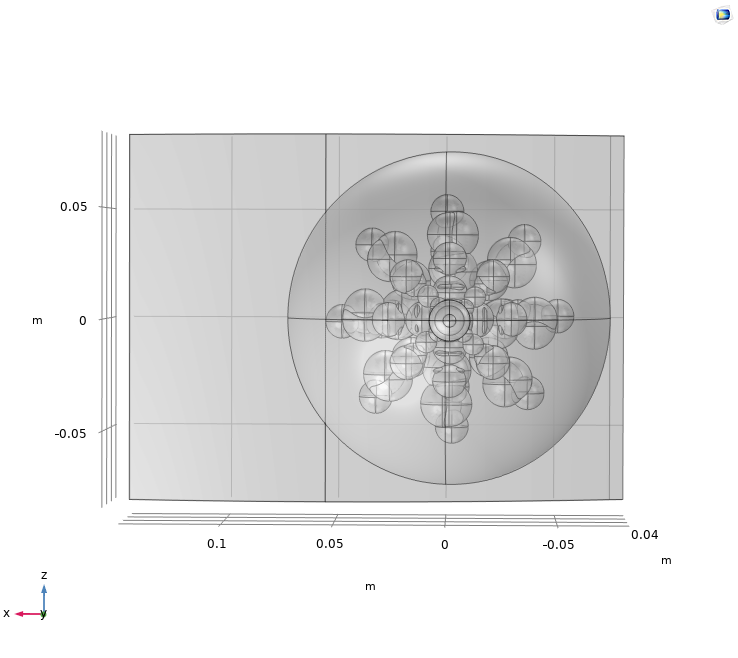
\includegraphics[width=\linewidth]{Figures/model_pictures/stage3_glandular/stage3_glandular_wide_anterior_offset055.png}}{\fbox{\parbox[c][0.2\textheight][c]{0.9\linewidth}{\centering Placeholder: wide glandular spread}}}
\caption{Wide}
\end{subfigure}
\caption{Stage 3 glandular distribution variants. The reference case is used in the current anatomical route; compact and wide cases are useful for later spatial-distribution sensitivity.}
\label{fig:appendix_stage3_glandular_screens}
\end{figure}

\begin{figure}[H]
\centering
\begin{subfigure}{0.48\linewidth}
\centering
\IfFileExists{Figures/model_pictures/stage4_asymmetry_nipple/stage4_asymmetry_widthstretch_anterior_offset055.png}{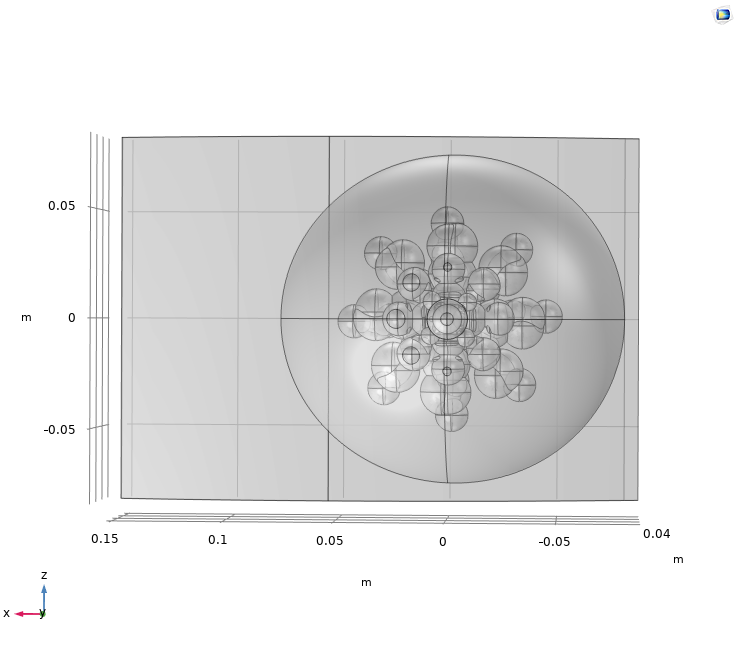
\includegraphics[width=\linewidth]{Figures/model_pictures/stage4_asymmetry_nipple/stage4_asymmetry_widthstretch_anterior_offset055.png}}{\fbox{\parbox[c][0.24\textheight][c]{0.9\linewidth}{\centering Placeholder: Stage 4 width/profile asymmetry}}}
\caption{Profile asymmetry}
\end{subfigure}
\hfill
\begin{subfigure}{0.48\linewidth}
\centering
\IfFileExists{Figures/model_pictures/stage4_asymmetry_nipple/stage4_asymmetry_nipplestretchsuperior_leftlateral_offset055.png}{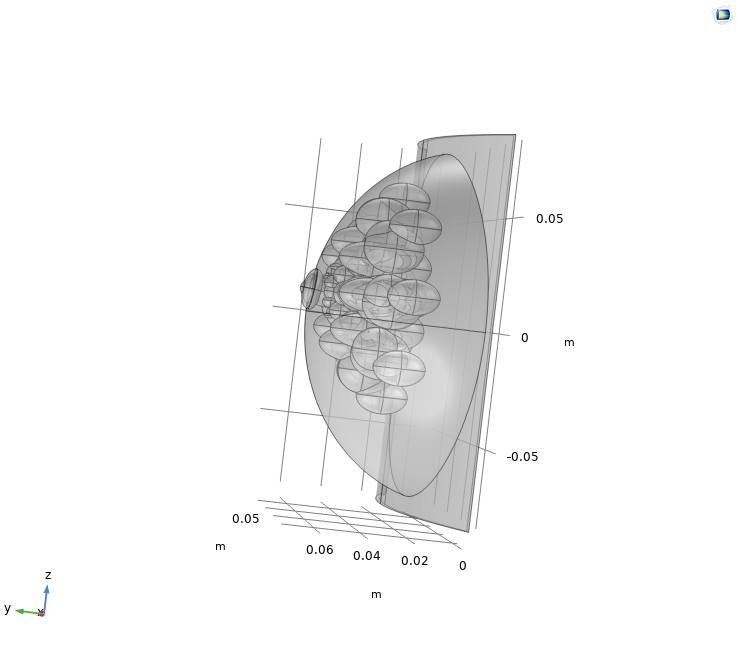
\includegraphics[width=\linewidth]{Figures/model_pictures/stage4_asymmetry_nipple/stage4_asymmetry_nipplestretchsuperior_leftlateral_offset055.png}}{\fbox{\parbox[c][0.24\textheight][c]{0.9\linewidth}{\centering Placeholder: Stage 4 nipple superior shift}}}
\caption{Nipple-position sensitivity}
\end{subfigure}
\caption{Stage 4 visual sensitivity cases. These figures are best used as geometry documentation rather than quantitative evidence until matched solved asymmetry runs are available.}
\label{fig:appendix_stage4_asymmetry_screens}
\end{figure}

\begin{figure}[H]
\centering
\IfFileExists{Figures/model_pictures/stage5_cooper/stage5_cooper_variants_schematic.png}{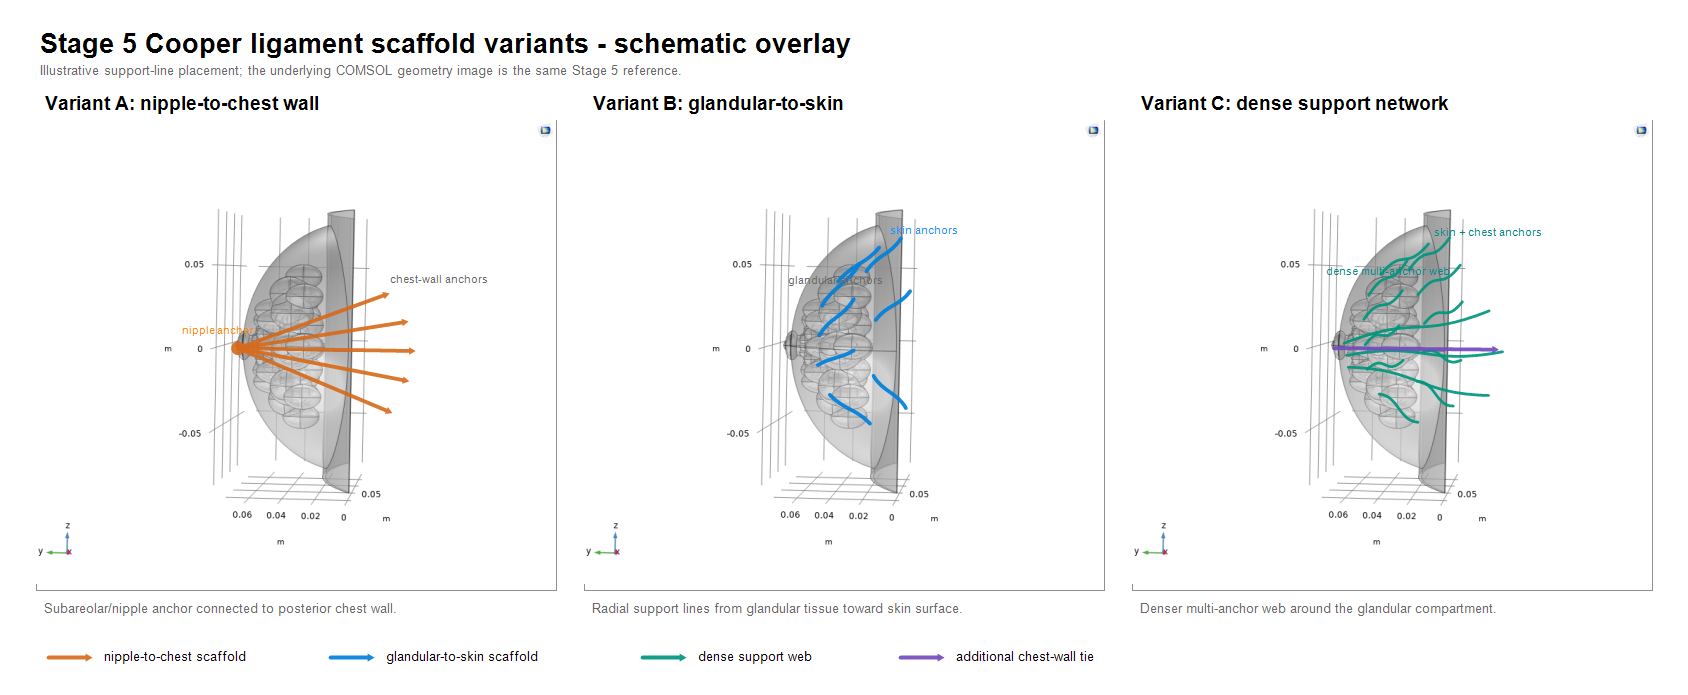
\includegraphics[width=0.95\linewidth]{Figures/model_pictures/stage5_cooper/stage5_cooper_variants_schematic.png}}{\fbox{\parbox[c][0.28\textheight][c]{0.85\linewidth}{\centering Placeholder: Stage 5 Cooper scaffold schematic}}}
\caption{Stage 5 Cooper-support schematic. This is an explanatory figure for the tested support concepts; current quantitative results should still use the stable no-Cooper control unless a Cooper variant solves robustly.}
\label{fig:appendix_stage5_cooper_schematic}
\end{figure}

\begin{figure}[H]
\centering
\begin{subfigure}{0.32\linewidth}
\centering
\IfFileExists{Figures/model_pictures/stage6_tumor/stage6_tumor_small_central_sideview.png}{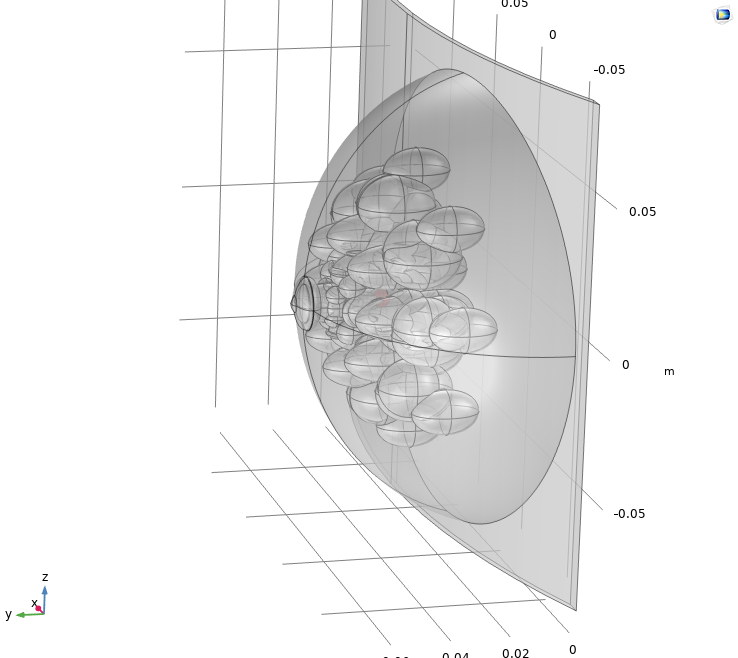
\includegraphics[width=\linewidth]{Figures/model_pictures/stage6_tumor/stage6_tumor_small_central_sideview.png}}{\fbox{\parbox[c][0.2\textheight][c]{0.9\linewidth}{\centering Placeholder: small central tumor}}}
\caption{Small central}
\end{subfigure}
\hfill
\begin{subfigure}{0.32\linewidth}
\centering
\IfFileExists{Figures/model_pictures/stage6_tumor/stage6_tumor_small_upper_outer_leftlateral.png}{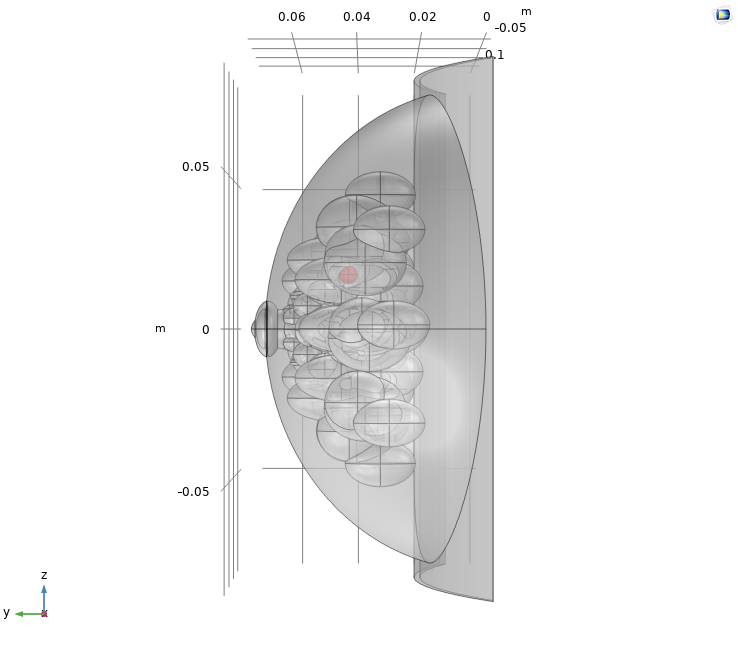
\includegraphics[width=\linewidth]{Figures/model_pictures/stage6_tumor/stage6_tumor_small_upper_outer_leftlateral.png}}{\fbox{\parbox[c][0.2\textheight][c]{0.9\linewidth}{\centering Placeholder: small upper-outer tumor}}}
\caption{Small upper-outer}
\end{subfigure}
\hfill
\begin{subfigure}{0.32\linewidth}
\centering
\IfFileExists{Figures/model_pictures/stage6_tumor/stage6_tumor_large_central_sideview.png}{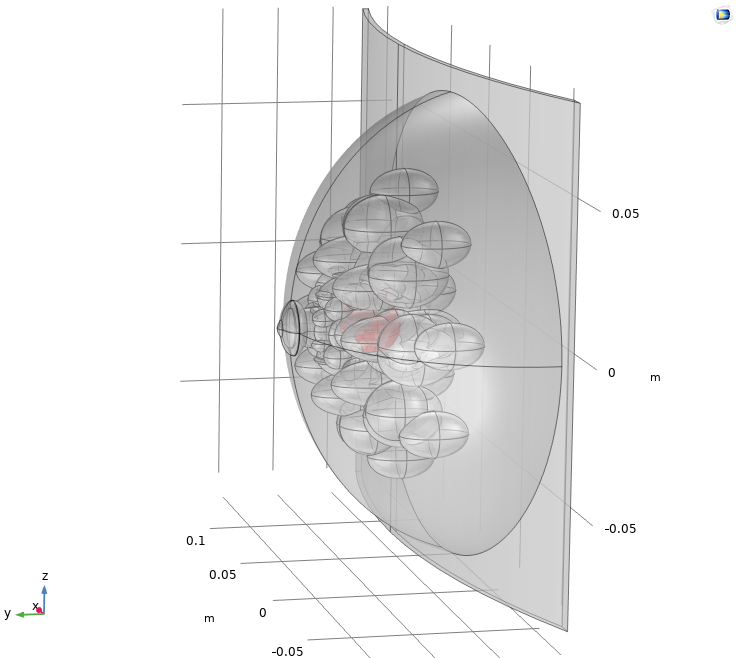
\includegraphics[width=\linewidth]{Figures/model_pictures/stage6_tumor/stage6_tumor_large_central_sideview.png}}{\fbox{\parbox[c][0.2\textheight][c]{0.9\linewidth}{\centering Placeholder: large central tumor}}}
\caption{Large central}
\end{subfigure}
\caption{Stage 6 tumor-placement examples. These screenshots support visual validation of lesion location and scale before the cases are used for dynamic interpretation.}
\label{fig:appendix_stage6_tumor_screens}
\end{figure}
